\subsection{单孤子的三场分布}
本节对第 \ref{ch:rhp} 节证明的一轨道无反射解作数值求值. 图中使用规范变换前的场 $\widetilde q,\widetilde p,\eta$, 它们由 \eqref{eq:original-fields} 恢复. 取参数
\begin{equation}\label{eq:numerical-parameters}
q_0=1,\qquad a=2,\qquad\eta_0=0.6,\qquad
\alpha=1,\qquad\beta=0.1,\qquad b=1.5,
\end{equation}
范数常数由式 \eqref{eq:onec} 给定, 场值由四维留数系统及无穷远、共振点的重构公式计算, 不作 HMB 方程的数值离散. 图 \ref{fig:one} 展示光场的局域振荡及同一区域内的极化和粒子数反转.

\paragraph{先把所有固定参数逐项代入.}
由 $b>q_0$ 的条件, 本例 $1.5>1$ 合法. 原文在式 \eqref{eq:imaginarypoint} 定义的三个量分别为
\begin{align*}
\kappa&=\sqrt{b^2-q_0^2}=\sqrt{1.5^2-1^2}
=\sqrt{2.25-1}=\dfrac{\sqrt{5}}{2},\\
 W&=b+\kappa=\dfrac{3}{2}+\dfrac{\sqrt{5}}{2}
=\dfrac{3+\sqrt{5}}{2},\\
h_0&=\dfrac{q_0}{W}=\dfrac{2}{3+\sqrt{5}}
=\dfrac{2(3-\sqrt{5})}{(3+\sqrt{5})(3-\sqrt{5})}
=\dfrac{3-\sqrt{5}}{2}.
\end{align*}
这里是把原文已有量求值, 没有引入新的代换. 因而两个 $D_+$ 离散零点为
\[
\zeta_1=\dfrac{\ii(3+\sqrt{5})}{2},\qquad
\zeta_2=-\dfrac{\ii(3-\sqrt{5})}{2}.
\]
它们各自的共轭给出另外两个谱点. 外部零点绝对值大于1, 内部零点绝对值小于1, 正好与第6部分的轨道结构相符. 范数常数的具体代入为
\[
c_1=\dfrac{4\ii\cdot\dfrac{\sqrt{5}}{2}}
{1+\left(\dfrac{3-\sqrt{5}}{2}\right)^2},\qquad
c_2=-\left(\dfrac{3-\sqrt{5}}{2}\right)^2c_1.
\]
共同相位的频率和 Bloch 长度平方则为
\begin{align*}
\Omega&=-\alpha q_0^2+\dfrac{2\eta_0}{a}
=-1+\dfrac{2\cdot0.6}{2}=-0.4,\\
\eta_0^2\left(1+\dfrac{q_0^2}{a^2}\right)
&=0.6^2\left(1+\dfrac{1}{4}\right)
=0.36\cdot1.25=0.45.
\end{align*}
所以两端原场具体是
\[
\widetilde q_{\rm bg}=e^{0.4\ii t},\qquad
\widetilde p_{\rm bg}=-0.3\ii e^{0.4\ii t},\qquad
\eta_{\rm bg}=0.6.
\]

\paragraph{一个网格点上的求值顺序.}
先固定所要画图的原变量 $x,t$, 代入原文的 $s=\kappa[x-F(\ii b)t]$ 和 $T=e^{2s}$. 接着计算 $C_1=c_1T$、$C_2=-h_0^2c_1\conj{T}$, 再把这两个数与固定的谱点代入式 \eqref{eq:finite1}--\eqref{eq:finite2}. 两个向量分量分别对应同一个四阶标量系数矩阵的一个右端, 所以解两次同一个系数矩阵即可得到四个正则列. 把它们代回式 \eqref{eq:partialfraction}, 就可以在任意普通谱点求 $M$. 光场用式 \eqref{eq:qfinite}; 介质用式 \eqref{eq:RfromM}. 最后乘回 $e^{-\ii\Omega t}$ 得到原物理复场. 此过程只是在不同 $x,t$ 上对解析表达式求值, 没有用相邻网格点近似偏导数来推进 PDE.

\paragraph{图中的三个纵坐标为什么这样取.}
复数不能直接作为通常三维实坐标的高度. 图中光场和极化取非负实数 $|\widetilde q|$ 与 $|\widetilde p|$, 反转取实值 $\eta$. 因共同相位的模为1,
\[
|\widetilde q|=|e^{-\ii\Omega t}q|=|q|,\qquad
|\widetilde p|=|-e^{-\ii\Omega t}R_{12}|=|R_{12}|.
\]
所以恢复共同相位会改变复场的实部与虚部, 却不会改变这两张模长曲面. Bloch 恒等式还给出逐点核验关系
\[
|\widetilde p|^2+\eta^2=0.45,
\qquad |\eta|\le\sqrt{0.45},\qquad
|\widetilde p|\le\sqrt{0.45}.
\]
这不是说两个介质分量各自保持常数, 而是说它们的平方和固定.
\begin{figure}[!htbp]
\centering
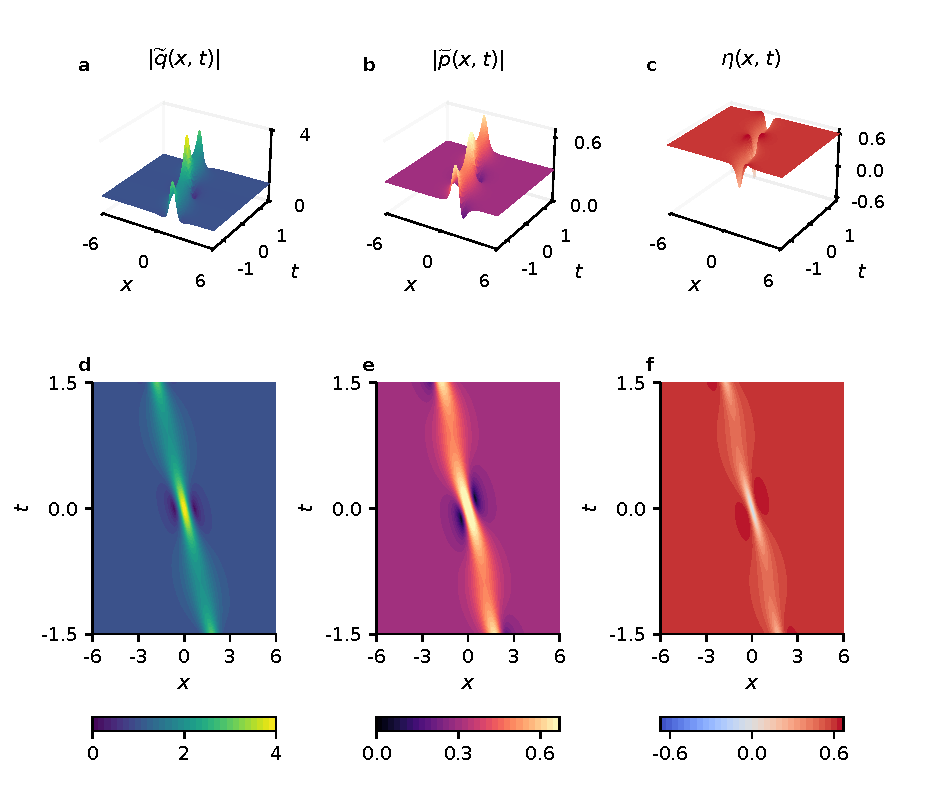
\includegraphics[width=\textwidth]{figures/one-soliton-fields.pdf}
\caption{单轨道物理三场 $|\widetilde q|,|\widetilde p|,\eta$ 的曲面 (上排) 与等值图 (下排). 参数见 \eqref{eq:numerical-parameters}; $x\in\lbrack-6,6\rbrack$, $t\in\lbrack-1.5,1.5\rbrack$.}
\label{fig:one}
\end{figure}

\FloatBarrier
\subsection{传播速度与内部振荡}
将背景传播因子分解为
\begin{align}
A_b=\operatorname{Re}F(\ii b)
&=-4\beta b^2-2\beta q_0^2-\dfrac{\eta_0}{a^2+b^2},\label{eq:velocity}\\
B_b=\operatorname{Im}F(\ii b)
&=-\alpha b-\dfrac{\eta_0b}{a(a^2+b^2)}.\label{eq:frequency}
\end{align}
\paragraph{传播函数实部和虚部的全部计算.}
从式 \eqref{eq:F} 原封不动代入 $k=\ii b$:
\begin{align*}
F(\ii b)
&=4\beta(\ii b)^2-\alpha\ii b-2\beta q_0^2
+\dfrac{\eta_0}{a(\ii b-a)}\\
&=-4\beta b^2-\ii\alpha b-2\beta q_0^2
+\dfrac{\eta_0(-a-\ii b)}{a(\ii b-a)(-a-\ii b)}.
\end{align*}
分母中
\[
(\ii b-a)(-a-\ii b)
=-\ii ab+b^2+a^2+\ii ab=a^2+b^2.
\]
所以有理项恰为
\[
\dfrac{\eta_0}{a(\ii b-a)}
=-\dfrac{\eta_0}{a^2+b^2}
-\ii\dfrac{\eta_0b}{a(a^2+b^2)}.
\]
其余各项的实虚性都已显现. 把没有 $\ii$ 的项与含 $\ii$ 的项分别合并, 就得到式 \eqref{eq:velocity}--\eqref{eq:frequency}. 因为所有参数为实数, 这里无需再对任何系数取实部或虚部. 同时
\[
F(-\ii b)=A_b-\ii B_b=\conj{F(\ii b)},
\]
与第8部分使用的两个 $D_+$ 点的指数关系一致.

于是 $s=\kappa X-\ii\kappa B_bt$, 其中 $X=x-A_bt$. 显式矩阵 $P$ 关于 $x,t$ 的依赖由
\[
T=e^{2s}=e^{2\kappa X}e^{-2\ii\kappa B_bt}
\]
确定. 固定 $X$ 时, 若 $B_b\ne0$, 去相位三场具有周期
\begin{equation}\label{eq:internal-period}
T_t=\dfrac{\pi}{\kappa|B_b|}.
\end{equation}
\paragraph{包络移动和内部振荡怎样从同一个指数读出.}
不另设坐标, 先直接在原变量中展开:
\begin{align*}
s&=\kappa\{x-(A_b+\ii B_b)t\}
=\kappa(x-A_bt)-\ii\kappa B_bt,\\
2s&=2\kappa(x-A_bt)-2\ii\kappa B_bt,\\
|T|&=\left|e^{2\kappa(x-A_bt)}e^{-2\ii\kappa B_bt}\right|
=e^{2\kappa(x-A_bt)}.
\end{align*}
原文的 $X=x-A_bt$ 仅把已经出现的表达式命名, 本册没有额外变换. 要使 $|T|$ 保持相同, 就要保持 $x-A_bt$ 相同, 因而中心线是 $x=A_bt$. 同时比较 $t$ 与 $t+T_t$ 且沿这条同速轨迹移动 $x$, 有
\begin{align*}
T(x+A_bT_t,t+T_t)
&=e^{2\kappa[x+A_bT_t-A_b(t+T_t)]}
e^{-2\ii\kappa B_b(t+T_t)}\\
&=T(x,t)e^{-2\ii\kappa B_bT_t}.
\end{align*}
要让这个额外因子等于1, 其指数的相位必须是 $2\pi$ 的整数倍. 取正的完整相位周期,
\[
2\kappa|B_b|T_t=2\pi
\quad\Longrightarrow\quad
T_t=\dfrac{\pi}{\kappa|B_b|}.
\]
$P$ 是 $T,\conj{T}$ 的有理函数, $N(a)$ 是 $P$ 的矩阵多项式, 所以它们及规范三场都在这个平移后恢复原值. 这里的 $T_t$ 是原文给周期起的名称, 不是偏导数 $\partial_tT$. 本段证明了该值是一个周期, 不需要另行断言所有特殊参数下都没有更小周期.

若 $\alpha=-\dfrac{\eta_0}{a(a^2+b^2)}$, 则 $B_b=0$, 去相位三场仅依赖 $X$. 原场的模 $|\widetilde q|,|\widetilde p|$ 和反转 $\eta$ 也具有周期 \eqref{eq:internal-period}; 复场 $\widetilde q,\widetilde p$ 具有同一随动周期当且仅当 $\Omega T_t\in2\pi\mathbb Z$.

\paragraph{消除内部振荡与恢复共同相位.}
由 $b>q_0>0$ 可除以 $b$. 将 $B_b$ 的表达式设为零, 逐步得到
\begin{align*}
0&=-\alpha b-\dfrac{\eta_0b}{a(a^2+b^2)},\\
0&=-\alpha-\dfrac{\eta_0}{a(a^2+b^2)},\\
\alpha&=-\dfrac{\eta_0}{a(a^2+b^2)}.
\end{align*}
此时 $s$ 没有随 $t$ 单独变化的虚部, 所有规范场仅通过 $x-A_bt$ 变化. 这里不能把含 $|B_b|$ 的周期公式代入零分母; 正确结论是内部振荡消失.

当 $B_b\ne0$ 时, 规范场在一次随动周期后恢复, 原复光场还多出
\[
\dfrac{e^{-\ii\Omega(t+T_t)}}{e^{-\ii\Omega t}}
=e^{-\ii\Omega T_t}.
\]
由于 $q$ 有非零端态 $q_0$, 若要求整个复光场在同一次平移后恢复, 该因子必须为1. 这等价于 $\Omega T_t\in2\pi\mathbb Z$. 极化同理. 模长则不受这个因子影响, 反转本来就没有共同相位.

由 $P^2=P=P^\dagger$ 和 $\tr P=1$, 有 $|P_{12}|^2=P_{11}(1-P_{11})\le\dfrac{1}{4}$. 因而
\begin{equation}\label{eq:amplitude-bound}
|\widetilde q(x,t)|\le q_0+2b,\qquad |\widetilde q(0,0)|=q_0+2b.
\end{equation}
后一等式使用 $T(0,0)=1$ 和 $P_{12}(0,0)=\dfrac{1}{2}$. $P$ 在 $X\to\pm\infty$ 时趋于端态投影, 修正项为 $O(e^{-2\kappa|X|})$, 所以局域化尺度由 $\kappa$ 决定.

\paragraph{振幅估计每一步的不等式.}
Hermitian 性给出 $P_{21}=\conj{P_{12}}$. 取 $P^2=P$ 的第1行第1列:
\begin{align*}
P_{11}^2+P_{12}P_{21}&=P_{11},\\
|P_{12}|^2&=P_{11}-P_{11}^2
=\dfrac{1}{4}-\left(P_{11}-\dfrac{1}{2}\right)^2\le\dfrac{1}{4}.
\end{align*}
$P_{11}$ 为实数, 所以平方项非负, 从而 $|P_{12}|\le\dfrac{1}{2}$. 取式 \eqref{eq:finalfields} 中光场的模并应用三角不等式,
\begin{align*}
|\widetilde q|
&=\left|e^{-\ii\Omega t}(-q_0-4bP_{12})\right|
=|-q_0-4bP_{12}|\\
&\le q_0+4b|P_{12}|
\le q_0+2b.
\end{align*}
在 $x=t=0$ 时, 原文 $s=0$, $T=1$. 由 $\Delta_-=|T-h_0|^2+|1-h_0T|^2$,
\[
\Delta_-(0,0)=2(1-h_0)^2,
\qquad
P_{12}(0,0)=\dfrac{(1-h_0)(1-h_0)}{2(1-h_0)^2}=\dfrac{1}{2}.
\]
于是 $\widetilde q(0,0)=-q_0-2b$ 是负实数, 它的模正好达到上界. 本例等于 $1+2\cdot1.5=4$.

\paragraph{在原点同时检查两个介质分量.}
原点 $P$ 的四个元均为 $\dfrac{1}{2}$, 故式 \eqref{eq:Nfactor} 中的 $N(a)$ 在这里为
\[
N(a)=aI+\ii b(I-2P)
=\begin{pmatrix}a&-\ii b\\-\ii b&a\end{pmatrix}.
\]
将这四个元代入式 \eqref{eq:etacomponent}--\eqref{eq:pcomponent}:
\begin{align*}
\eta(0,0)
&=\dfrac{\eta_0}{a^2+b^2}
\left[a^2-b^2+\dfrac{\ii q_0}{a}
\{a(\ii b)-(-\ii b)a\}\right]\\
&=\dfrac{\eta_0}{a^2+b^2}(a^2-b^2-2bq_0),\\
\widetilde p(0,0)
&=\dfrac{\eta_0}{a^2+b^2}
\left[a(\ii b)-(-\ii b)a
+\dfrac{\ii q_0}{a}\{a^2-(-\ii b)(\ii b)\}\right]\\
&=\dfrac{\ii\eta_0}{a^2+b^2}
\left[2ab+\dfrac{q_0}{a}(a^2-b^2)\right].
\end{align*}
本例 $a^2+b^2=4+2.25=6.25$, 故
\begin{align*}
\eta(0,0)&=\dfrac{0.6}{6.25}(4-2.25-3)=-0.12,\\
\widetilde p(0,0)&=\dfrac{0.6\ii}{6.25}
\left[6+\dfrac{4-2.25}{2}\right]=0.66\ii,\\
|\widetilde p(0,0)|^2+\eta(0,0)^2
&=0.66^2+(-0.12)^2=0.4356+0.0144=0.45.
\end{align*}
因此图中中心处的介质偏离背景, 但仍严格位于同一个 Bloch 长度约束上.

\paragraph{指数衰减的量级为何是这个指数.}
由原文的 $P$ 公式, 当 $|T|\to0$ 时, 分子和分母都可以按 $T,\conj{T}$ 展开. 分母常数项是 $1+h_0^2>0$, 所以 $P-P_-$ 的每个元都是 $O(|T|)$. 当 $|T|\to\infty$ 时, 把分子分母同时除以 $|T|^2$, 常数主项给出 $P_+$, 其余是 $O(|T|^{-1})$. 又
\[
|T|=e^{2\kappa X},\qquad
|T|^{-1}=e^{-2\kappa X}.
\]
所以 $X\to-\infty$ 与 $X\to+\infty$ 的误差统一是 $O(e^{-2\kappa|X|})$. 光场是 $P$ 的线性表达式, 介质是 $P$ 的光滑有理矩阵表达式且分母 $a^2+b^2>0$, 因此三场保持同样的衰减量级.

参数 \eqref{eq:numerical-parameters} 给出 $A_b=-1.196$、$B_b=-1.572$ 和 $T_t\approx1.78748466439$. 图 \ref{fig:dynamics} 左图比较 $t=0,\dfrac{T_t}{4},\dfrac{T_t}{2}$ 时的随动截面; 右图比较 $\alpha=-0.048,0.5,1$ 时的中心光场模. 后两者的周期分别约为 $3.41840132897$ 和 $1.78748466439$, 而 $\alpha=-0.048$ 对应行波.
\paragraph{这些小数怎样算出.}
本例公共分母为 $a^2+b^2=6.25$. 逐项代入得
\begin{align*}
A_b&=-4\cdot0.1\cdot1.5^2-2\cdot0.1\cdot1^2-\dfrac{0.6}{6.25}\\
&=-0.9-0.2-0.096=-1.196,\\
B_b&=-1\cdot1.5-\dfrac{0.6\cdot1.5}{2\cdot6.25}
=-1.5-0.072=-1.572,\\
T_t&=\dfrac{\pi}{\dfrac{\sqrt{5}}{2}\cdot1.572}
\approx1.78748466439.
\end{align*}
当只把 $\alpha$ 改成 $0.5$ 时, $A_b$ 的表达式中没有 $\alpha$, 所以传播速度不变, 而
\[
B_b=-0.5\cdot1.5-0.072=-0.822,\qquad
T_t=\dfrac{\pi}{\dfrac{\sqrt{5}}{2}\cdot0.822}
\approx3.41840132897.
\]
当 $\alpha=-0.048$ 时,
\[
B_b=-(-0.048)\cdot1.5-0.072=0.072-0.072=0.
\]
同一个数也由临界参数式给出:
\[
-\dfrac{\eta_0}{a(a^2+b^2)}=-\dfrac{0.6}{2\cdot6.25}=-0.048.
\]
因此三条中心曲线的差别是内部振荡变化, 不是中心沿 $x$ 方向的移动速度变化. 图左在固定随动位置比较不同 $t$ 的截面, 正是为了能直接看见这个内部变化.
\begin{figure}[htbp]
\centering
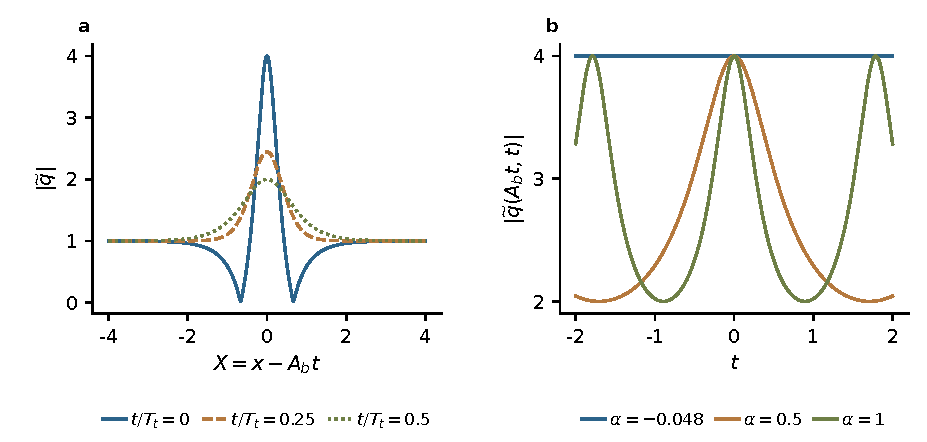
\includegraphics[width=\textwidth]{figures/one-soliton-dynamics.pdf}
\caption{单轨道光场的局域化与内部振荡. (a) 参数 \eqref{eq:numerical-parameters} 下的随动截面. (b) 改变 $\alpha$ 时 $|\widetilde q(A_bt,t)|$ 的变化, 其余参数固定.}
\label{fig:dynamics}
\end{figure}

\FloatBarrier
\subsection{参数影响与数值验证}
$\beta$ 改变式 \eqref{eq:velocity} 中的传播速度, 而不改变式 \eqref{eq:frequency} 中的内部频率. 图 \ref{fig:velocity} 取 $\beta=0,0.15$, 相应的 $A_b$ 为 $-0.096,-1.746$; 两者均有 $B_b=-1.572$ 和相同的随动周期. 虚线 $x=A_bt$ 表示中心轨迹.
\paragraph{分离两个参数作用的直接计算.}
在当前参数下, 速度对 $\beta$ 的依赖直接合并成
\[
A_b=-4\beta\cdot2.25-2\beta-0.096=-11\beta-0.096.
\]
代入图中两个取值得
\[
\beta=0:\quad A_b=-0.096,\qquad
\beta=0.15:\quad A_b=-11\cdot0.15-0.096=-1.746.
\]
两者都是负数, 所以 $t$ 增加时中心向更小的 $x$ 传播. 在固定 $q_0,a,\eta_0,b$ 下, 对原表达式求参数导数还可直接看出
\[
\dfrac{\partial A_b}{\partial\beta}=-4b^2-2q_0^2,\qquad
\dfrac{\partial B_b}{\partial\beta}=0,\qquad
\dfrac{\partial A_b}{\partial\alpha}=0,\qquad
\dfrac{\partial B_b}{\partial\alpha}=-b.
\]
因此在这个一轨道族中, 改变 $\beta$ 直接改变包络速度, 改变 $\alpha$ 直接改变内部振荡频率. 这几条参数偏导数只是原式的求导, 不需要额外的扰动理论. $\alpha$ 还通过 $\Omega$ 改变原复场的共同相位; 模长图没有显示这一相位变化.
\begin{figure}[htbp]
\centering
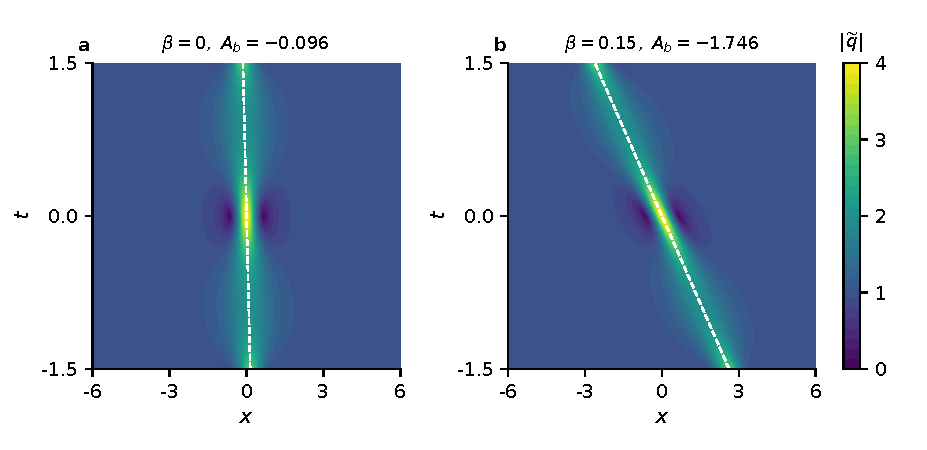
\includegraphics[width=\textwidth]{figures/one-soliton-velocity.pdf}
\caption{改变 $\beta$ 时的光场传播速度. 两图分别取 $\beta=0,0.15$, 其余参数同 \eqref{eq:numerical-parameters}; 白色虚线为 $x=A_bt$.}
\label{fig:velocity}
\end{figure}

对参数 \eqref{eq:numerical-parameters}, 采用 70 位十进制精度求解留数系统并对重构场求导, 得到表 \ref{tab:direct-residuals}. 导数由重构表达式直接计算. 双精度绘图实现与高精度实现的三个场在相同样点上的差均小于 $10^{-14}$; 等值图网格上的 Bloch 长度平方偏差及 $\eta$ 虚部均小于 $10^{-14}$. 两端 $x=\pm30$ 的三场误差均小于 $5.02\times10^{-29}$.
\begin{table}[htbp]
\centering
\caption{单轨道三场的高精度核验, 表内为样点最大绝对残差的向上舍入值}
\label{tab:direct-residuals}
\begin{tabular}{lc}
\toprule 检验对象 & 最大绝对误差\\\midrule
光场方程 & $1.87\times10^{-69}$\\
极化方程 & $8.26\times10^{-71}$\\
粒子数反转方程 & $1.50\times10^{-70}$\\
空间 Lax 方程 & $4.82\times10^{-70}$\\
时间 Lax 方程 & $1.95\times10^{-69}$\\
两共振原像的介质重构 & $1.12\times10^{-71}$\\
Bloch 长度平方 & $4.77\times10^{-72}$\\
\bottomrule
\end{tabular}
\end{table}

\paragraph{表中各行的残差究竟怎样形成.}
先在一个给定样点计算场及其所需导数, 再把方程的全部项移到左边. 表中前三行对应以下三个复数或实数的绝对值:
\begin{align*}
\left|\widetilde q_t
-\ii\alpha\left(\dfrac{\widetilde q_{xx}}{2}+|\widetilde q|^2\widetilde q\right)
-\beta(\widetilde q_{xxx}+6|\widetilde q|^2\widetilde q_x)-2\widetilde p\right|,\\
\left|\widetilde p_x-2\eta\widetilde q+2\ii a\widetilde p\right|,\\
\left|\eta_x+\conj{\widetilde q}\widetilde p+\widetilde q\conj{\widetilde p}\right|.
\end{align*}
例如, 第二条的加号来自把原方程右端的 $-2\ii a\widetilde p$ 移到左边. 它不是把原方程改成了另一个符号约定. 对每个样点各算一次, 再对所有样点取最大值, 得到表中的最大绝对残差. 在精确算术下这三项都为零; 高精度计算中的小非零值来自有限精度求值和求导.

\paragraph{原场导数与规范场导数的关系.}
共同相位只依赖 $t$, 所以所有 $x$ 导数都可以把它提出. 按原文的光场和介质重构式,
\begin{align*}
\widetilde q_x&=-4b e^{-\ii\Omega t}\partial_xP_{12},\\
\widetilde q_{xx}&=-4b e^{-\ii\Omega t}\partial_x^2P_{12},\\
\widetilde q_{xxx}&=-4b e^{-\ii\Omega t}\partial_x^3P_{12},\\
\widetilde q_t
&=e^{-\ii\Omega t}\left[\ii\Omega(q_0+4bP_{12})-4b\partial_tP_{12}\right],\\
\widetilde p_x&=-e^{-\ii\Omega t}\partial_xR_{12},\qquad
\eta_x=\partial_xR_{11}.
\end{align*}
时间导数中必须保留 $\ii\Omega(q_0+4bP_{12})$; 漏掉它就会把原方程与规范后的方程混用. 原文已有指数的导数也可直接计算:
\begin{align*}
\partial_xT&=2\kappa T,&
\partial_x\conj{T}&=2\kappa\conj{T},\\
\partial_tT&=-2\kappa F(\ii b)T,&
\partial_t\conj{T}&=-2\kappa\conj{F(\ii b)}\conj{T}.
\end{align*}
在这组式子里使用 $\partial_tT$ 表示偏导, 避免与原文的周期名称 $T_t$ 混淆. 将这些导数用于 $P$ 的原有有理表达式, 就能以乘法法则和商法则生成场导数, 不必使用网格差分.
本节末尾的``投影矩阵与三场导数的逐项求值''继续写出这些商法则的三阶展开、全部投影元的一阶导数, 以及介质矩阵的逐元导数, 可按该顺序直接执行求值.

\paragraph{两条 Lax 残差的符号.}
由式 \eqref{eq:Mspace} 及 $\phi=Me^{\ii\theta\sg}$, 对修正矩阵计算的两条残差是
\[
M_x-UM-\ii\lambda M\sg,\qquad
M_t-VM+\ii\lambda F M\sg.
\]
空间式的右乘项是负号移到左边, 时间式则因 $\theta_t=\lambda F$ 带相反的符号. 对每个谱测试点先取每个矩阵元绝对值的最大值, 再跨样点取最大值, 即得到表中两条 Lax 行. 两共振原像的核验则分别用 $z_a^+$、$z_a^-$ 代入式 \eqref{eq:RfromM}, 取两个矩阵之差的最大元绝对值. Bloch 行直接计算
\[
\left||\widetilde p|^2+\eta^2-
\eta_0^2\left(1+\dfrac{q_0^2}{a^2}\right)\right|.
\]

\paragraph{误差量级与边界检查怎样解释.}
70位十进制精度是内部运算的精度设定, 不是说每个结果都有70位相对有效数字. 对接近零的残差, 表格报告的是绝对误差. ``向上舍入''表示显示值不低于本次样点计算的最大值. 原文表格保留底稿的数值; 本详细版的复核结果另存于工程的检查报告中, 不把一次重跑得到的末位变化写成新的解析结论.
其中三条 PDE、两条 Lax 方程、留数系统和两共振重构的本次高精度结果保存在
\texttt{calculations/direct-rhp-results.json}; 原点三场、传播参数及指数因子保存在
\texttt{calculations/expanded-numerics-check.json}. 原文所述完整绘图网格误差按底稿保留, 本次没有重新生成全部网格和图像.

本例 $\kappa=\dfrac{\sqrt{5}}{2}$, 所以固定 $t$ 时理论端态衰减含有因子 $e^{-\sqrt{5}|x|}$. 在 $|x|=30$ 时,
\[
e^{-2\kappa\cdot30}=e^{-30\sqrt{5}}\approx7.36\times10^{-30}.
\]
这只是指数部分的数量级, 还要乘上依赖固定 $t$ 和场分量的有限系数, 所以不能直接把它当作三场误差的共同上界. 实际边界检查分别计算
\[
|\widetilde q-q_0e^{-\ii\Omega t}|,\qquad
\left|\widetilde p+\dfrac{\ii\eta_0q_0}{a}e^{-\ii\Omega t}\right|,\qquad
|\eta-\eta_0|.
\]
解析证明说明对所有允许参数和全部实 $x,t$ 的结构结论, 数值检查则检验本次实现是否在具体样点上正确执行了公式. 两者在本节中的作用由此区分.
